\chapter{Getting Started}

\emph{The text of this chapter was brought in with minimal filtering from Melissa's document, it needs a lot of editing to make it mesh with the rest of the document.}

\section{Examples of Use}

Here is, in order, the list of commands that can be run to create
data products from the MOC ``P19'' dataset (\emph{MJB: why is it
called P19??}).  You can obtain this dataset from
\emph{http://broxtronix.org/nasa/p19.tgz ??}, to ensure that your
installation is working properly.

Download the tarball and it will unpack into a \texttt{p19} directory.  Create an output directory to hold the results, and invoke the \texttt{stereo} program:

\begin{verbatim}
	mkdir results
	stereo E0201461.cub M0100115.cub results/p19
\end{verbatim}

You can look at the results by examining the disparity images. These
show the horizontal and vertical components of the matching offsets
for each pixel, and they can be a useful debugging tool if you want
to check how the stereo matcher performed for a given stereo pair:

\begin{verbatim}
	cd results
	disparitydebug p19-D.exr -o p19-D     
	disparitydebug p19-F.exr -o p19-F
\end{verbatim}

\emph{MJB: What exactly is being examined in the resultant images, what are users looking for?}

A 3D mesh can be built from the point cloud and viewed using the
\texttt{osgviewer} program:

\begin{verbatim}
	point2mesh p19-PC.tif p19-L.tif -o p19
	osgviewer p19.ive
\end{verbatim}

When the \texttt{osgviewer} starts, you may want to turn off the
lighting (hit the `L' key).

A gridded DEM with floating point pixels can also be built from the point cloud:

\begin{verbatim}
	point2dem --xyz-to-lonlat -r mars p19-PC.tif -n -o p19
\end{verbatim}

You can also orthoproject the raw satellite imagery onto the DEM during this step:

\begin{verbatim}
	point2dem --xyz-to-lonlat -r mars p19-PC.tif -o p19 --orthoimage p19-L.tif
\end{verbatim}

Finally, you can create colorized, shaded relief (or both) images from the DEM, using these Vision Workbench programs:

\begin{verbatim}
	colormap p19-DEM.tif -o p19-colorized.tif
	hillshade p19-DEM.tif -o p19-shaded.tif -e 25
	colormap p19-DEM.tif --shaded-relief-file p19-shaded.tif -o p19-color-shaded.tif
\end{verbatim}

Finally, you can run the Vision Workbench's \texttt{image2qtree} on any of the following files:

\begin{itemize}
\item p19-DEM-normalized.tif
\item p19-DRG.tif 
\item p19-shaded.tif
\item p19-colorized.tif
\item p19-shaded-colorized.tif
\end{itemize}


\section{Tutorial}

The following example will utilize images from the MOC dataset, P19.

When choosing image pairs to process, images that are taken along
the same groundtrack (usually from the same orbit) with similar
viewing angles/lighting conditions and significant surface coverage
overlap (~80\% is ideal) are the best suited for creating stereo
image pairs. Depending on the characteristics of the mission data
set and the individual images, the degree of acceptable variation
will differ. * Significant differences between image characteristics
increases the error propagated through to the resulting data products.

Images do NOT need to be map projected before processing with this
application. They SHOULD be photometrically calibrated (in whatever
fashion suits your purposes). They must also be converted to ISIS
.cub files.

After initial photometric calibration (if necessary), convert the
files to ISIS .cub files and unzip them. This sequence assumes that
you have downloaded your image files from the NASA PDS.

The two example images for P19 are \texttt{E0201461.cub} and 
\texttt{M0100115.cub}.

\begin{figure}
\begin{center}
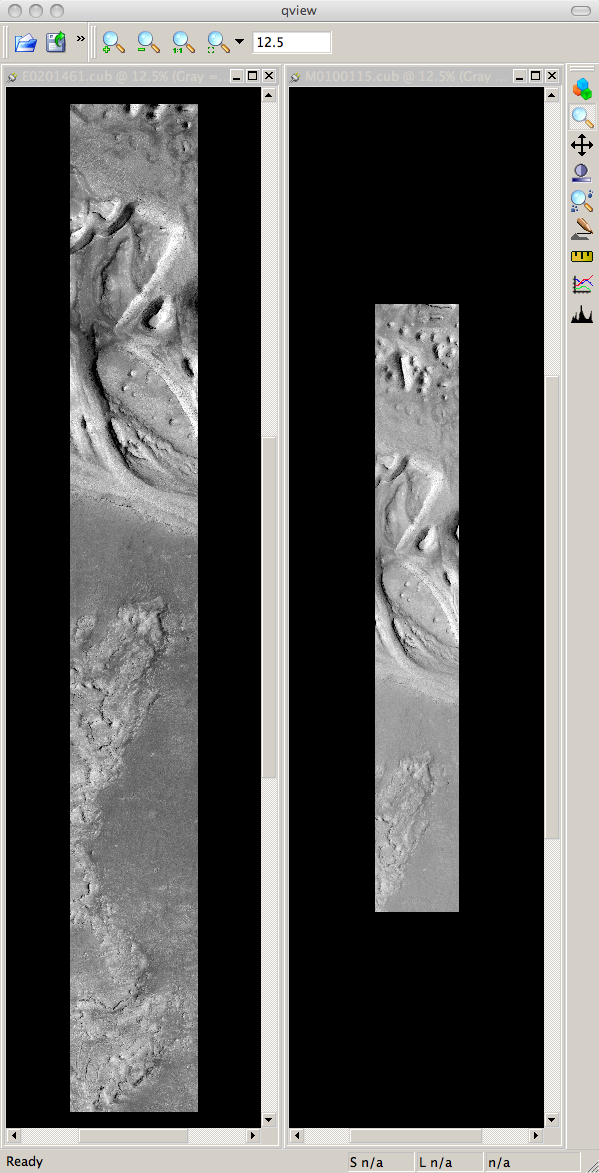
\includegraphics[width=4in]{images/p19-images.png}
\caption[P19 images open in qview]{
    \label{p19-images}
    This shows \texttt{E0201461.cub} and \texttt{M0100115.cub} open in
	ISIS's qview program.
    }
\end{center}
\end{figure}

Now that you have the two images, you can begin processing. 

The first step is the stereo processing. The \texttt{stereo} program is
designed to for automated tie point matching and stereo production.
Thus, you can use the basic program to create a stereo pair.

If you like, you should create a directory for the results of the processing. 

\begin{verbatim}
mkdir MOC_RESULTS
\end{verbatim}

Run \texttt{stereo} like this:

\begin{verbatim}
stereo E0201461.cub M0100115.cub MOC_RESULTS/E0201461_M0100115
\end{verbatim}

The \texttt{stereo} program requires a \texttt{stereo.default} file
which can be altered for your needs. You may find it useful to save
multiple versions of the \texttt{stereo.default} file for various
processing needs. If you need to do that, be sure to specify which
configuration file \texttt{stereo} should use (i.e., \texttt{stereo
–s my.stereo.default E0201461.cub M0100115.cub
MOC\_RESULTS/E0201461\_M0100115}).

\subsection*{Stereo Processing}

Stage 0 of the processing normalizes the two images and aligns them
(thus non-projected images are easier to work with) by locating
interest points and matching them in both images. The program is
designed to reject outlying interest points.

Stage 1 of the processing is correlation and the building of a disparity map. 

Stage 2 of the processing is refinement. 

Stage 3 is filtering and the creating of a ``good pixel'' map. 

Stage 4 is triangulation. The disparity map is processed to remove
the effects of interest point alignment and a 3D point cloud is
created.

If you would like to examine the images generated:

\begin{figure}
\begin{center}
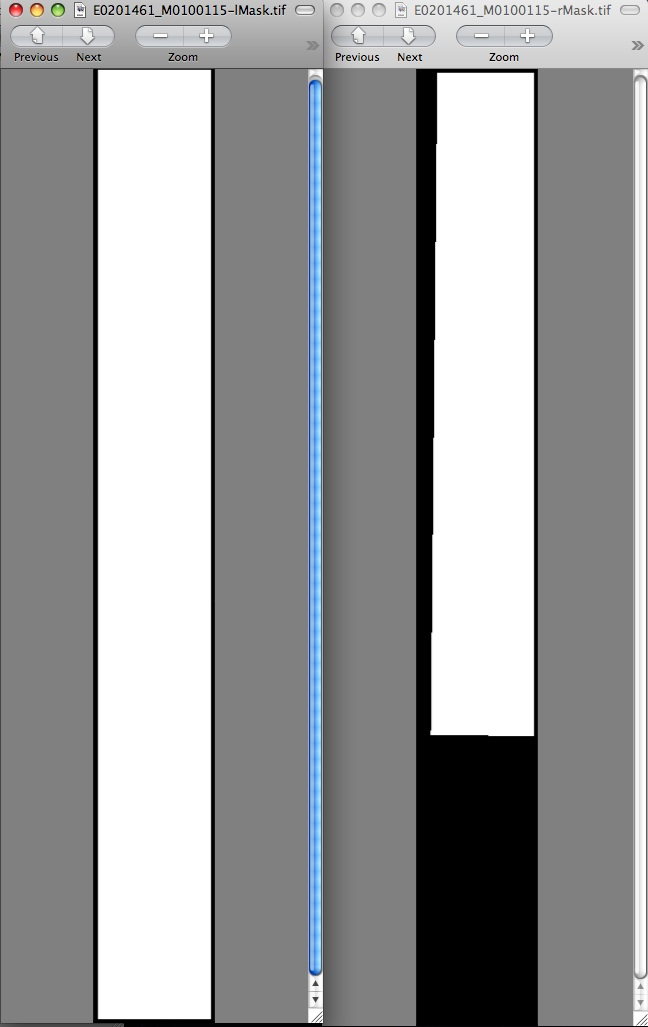
\includegraphics[width=3in]{images/p19-masks.png}
\caption[P19 images masks]{
    \label{p19-masks}
	The masks of pixels which are useful for alignment.
    }
\end{center}
\end{figure}

\begin{figure}
\begin{center}

\includegraphics[height=8in]{images/p19-goodpixel.png}
\caption[P19 good pixel image]{
    \label{p19-goodpixel}
	The Good Pixel map. 
	Red pixels are not useful for alignment. 
    }
\end{center}
\end{figure}

\begin{figure}
\begin{center}
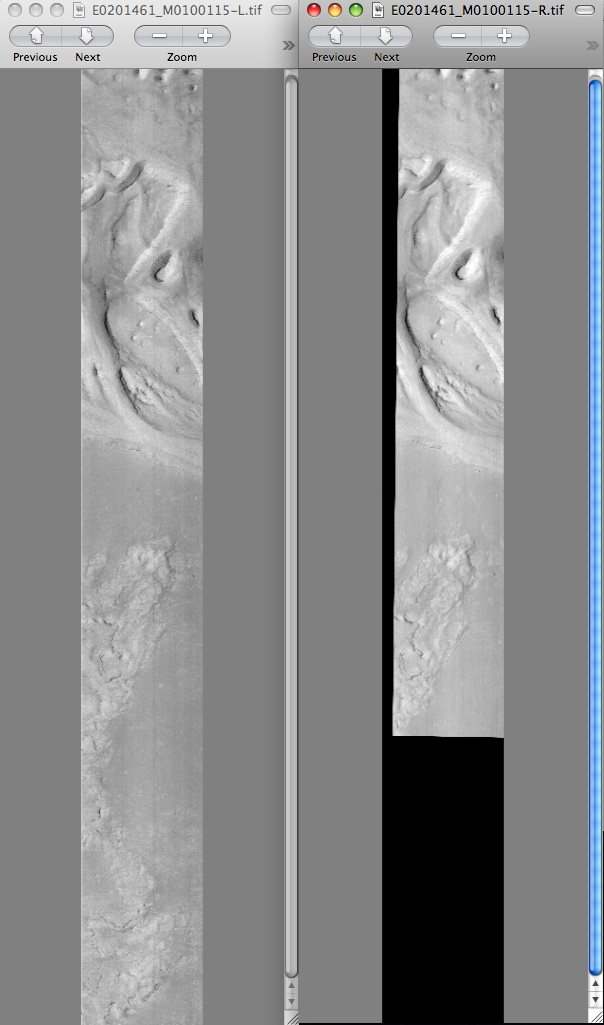
\includegraphics[width=3in]{images/p19-aligned.png}
\caption[P19 aligned image]{
    \label{p19-aligned}
	The left and right aligned images.
    }
\end{center}
\end{figure}

To begin an examination of the results, you must first examine the
disparity images. These images show the horizontal and vertical
components of the matching offsets for each pixel. They are
particularly useful if you want to check the performance of the
stereo matcher for any given stereo pair and they can be used as a
debugging tool.

Move into the directory that contains your results. 

\begin{verbatim}
cd MOC_RESULTS
\end{verbatim}

Invoke \texttt{disparitydebug} to examine the disparity files.

\begin{figure}
\begin{center}
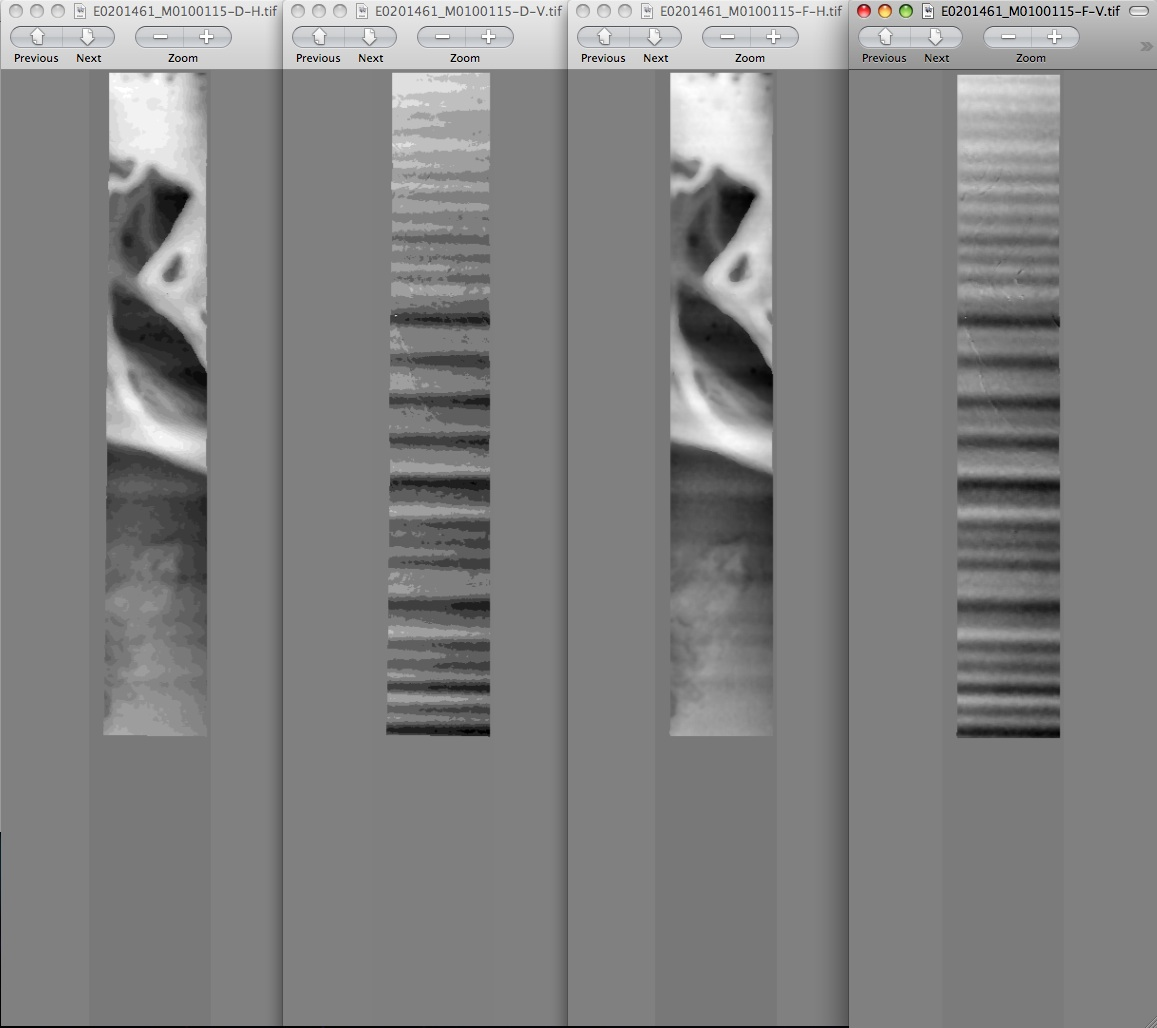
\includegraphics[width=4in]{images/p19-disparity.png}
\caption[P19 disparity images]{
    \label{p19-disparity}
	The disparity images.
    }
\end{center}
\end{figure}

The next step is to produce a 3D mesh with \texttt{point2mesh}.
This image can be viewed in the OSGViewer (Open Scene Graph Viewer,
distributed with the binary version of the Stereo Pipeline). This
feature utilizes the point cloud file and the left image file created
by \texttt{stereo}.

\begin{verbatim}
point2mesh E0201461_M0100115-PC.tif E0201461_M0100115-L.tif -o E0201461_M0100115
\end{verbatim}

This will create the file E0201461\_M0100115.ive, openable by OSGViewer.

The \texttt{point2dem} program creates a digital elevation model
(DEM) from the Point Cloud file.  You can specify a coordinate
system (e.g., latlon) and a reference spheroid (i.e., calculated
for the Moon or Mars). You also have the option of creating a
normalized DEM in addition to the automatically generated non-normalized
DEM.

\begin{verbatim}
point2dem --xyz-to-lonlat -r mars E0201461_M0100115-PC.tif -n -o E0201461_M0100115
\end{verbatim}

The \texttt{point2dem} program can also be used to orthoproject raw
satellite imagery onto the DEM. To do this, invoke \texttt{point2dem}
just as before, but add the \texttt{orthoimage} option and specify
the use of the Left image file as the texture file to use for the
projection.

\begin{verbatim}
point2dem --xyz-to-lonlat -r mars E0201461_M0100115-PC.tif -o E0201461_M0100115 --orthoimage E0201461_M0100115-L.tif 
\end{verbatim}

The \texttt{point2dem} program can be used in many different ways.
Be sure to explore all of the options.

\begin{figure}
\begin{center}
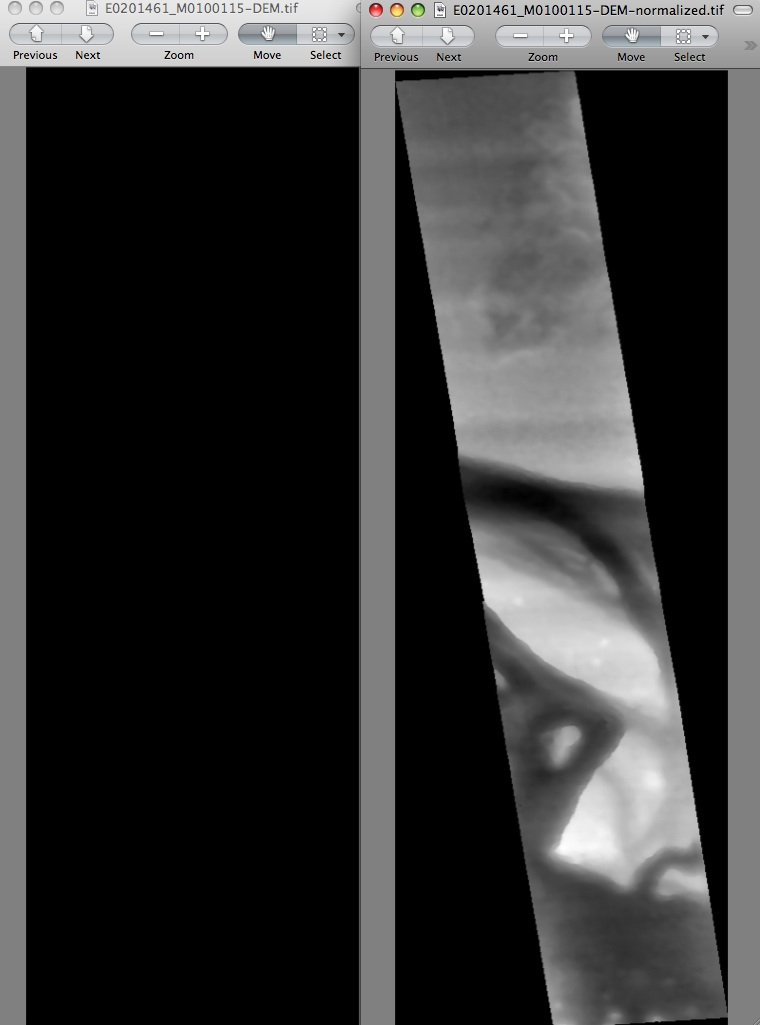
\includegraphics[width=4in]{images/p19-dems.png}
\caption[P19 dem images]{
    \label{p19-dems}
	The non-normalized and normalized DEMs. Note that the
	non-normalized version contains floating point pixel values
	and will not open in most image viewing programs which
	expect integer pixel values between 0 and 255 (which is
	what the normalized version does for you).
    }
\end{center}
\end{figure}

\begin{figure}
\begin{center}
\includegraphics[width=3in]{images/p19-ortho.png}
\caption[P19 orthophoto]{
    \label{p19-ortho}
	The left image orthoprojected onto the DEM.
    }
\end{center}
\end{figure}

Once you have generated a DEM, you can use the Vision Workbench's
\texttt{colormap} and \texttt{hillshade} tools to create colorized
and/or shaded relief images from the DEM.

To create a colorized version of the DEM, you need only specify the
DEM file to use:

\begin{verbatim}
colormap E0201461_M0100115-DEM.tif -o E0201461_M0100115-colorized.tif
\end{verbatim}

To create a hillshade of the DEM, you should specify the DEM file
to use. It is also advisable to explore the effects of altering the
elevation of the light source.

\begin{verbatim}
hillshade E0201461_M0100115-DEM.tif -o E0201461_M0100115-shaded.tif -e 25
\end{verbatim}
